
%??ds caption consistency?, but make captions "better" as per comments

\section{Magnetisation renormalisation methods}
\label{sec:magn-renorm-meth}

We compare renormalisation after every step with the methods used to achieve constant $\abs{\mv}$ in \nmag and \magpar.

We use fixed step BDF2 with step sizes of $\dtn = 0.1$ and a Newton-Raphson tolerance of $\ntol = 10^{-8}$ unless otherwise specified.
We choose BDF2 for these experiments because TR is equivalent to IMR for the undamped ODE LLG problem, and so could be expected to show some geometric integration properties.
In addition re-normalising the history values of TR, as described in \cref{sec:containing-renorm-impl} is more difficult as one of the stored values is a derivative (in our implementation, see \cref{eq:impl-tr}) which would need to be recalculated using the newly re-normalised magnetisation values.

\FloatBarrier
\subsection{Renormalisation after a tolerance}
\label{sec:renorm-after-toler}

\newcommand{\mltol}{\epsilon_{\mathrm{ml}}}

If the error in the magnetisation length, $\errml$, is less than the tolerance, $\mltol$, then nothing is done and the integration continues.
On the other hand if $\errml > \mltol$ then we set the current value of the magnetisation, $\mv_{n+1}$ to $\mv_{n+1}/\abs{\mv_{n+1}}$, additionally we perform the same renormalisation for each of the history values required by BDF2 (\ie $\mv_n$ and $\mv_{n-1}$).
\label{sec:containing-renorm-impl}


Note that all values are output after any renormalisation has taken place.
??ds should/could I change this?


\begin{figure}
  \centering
  \includegraphics[width=0.8\textwidth]{{{plots/tolrenorm-geom-properties/0.01-mlengtherrormaxesvstimes}}}
  \caption{
    Error in magnetisation length against time
    for the ODE LLG problem
    with $\dampc = 0.01$.
    The legend indicates the values of $\mltol$, the tolerance on the magnetisation length after which the magnetisation is re-normalised.
  }
  \label{fig:renorm-tol-ml-err}
\end{figure}

\begin{figure}
  \centering
  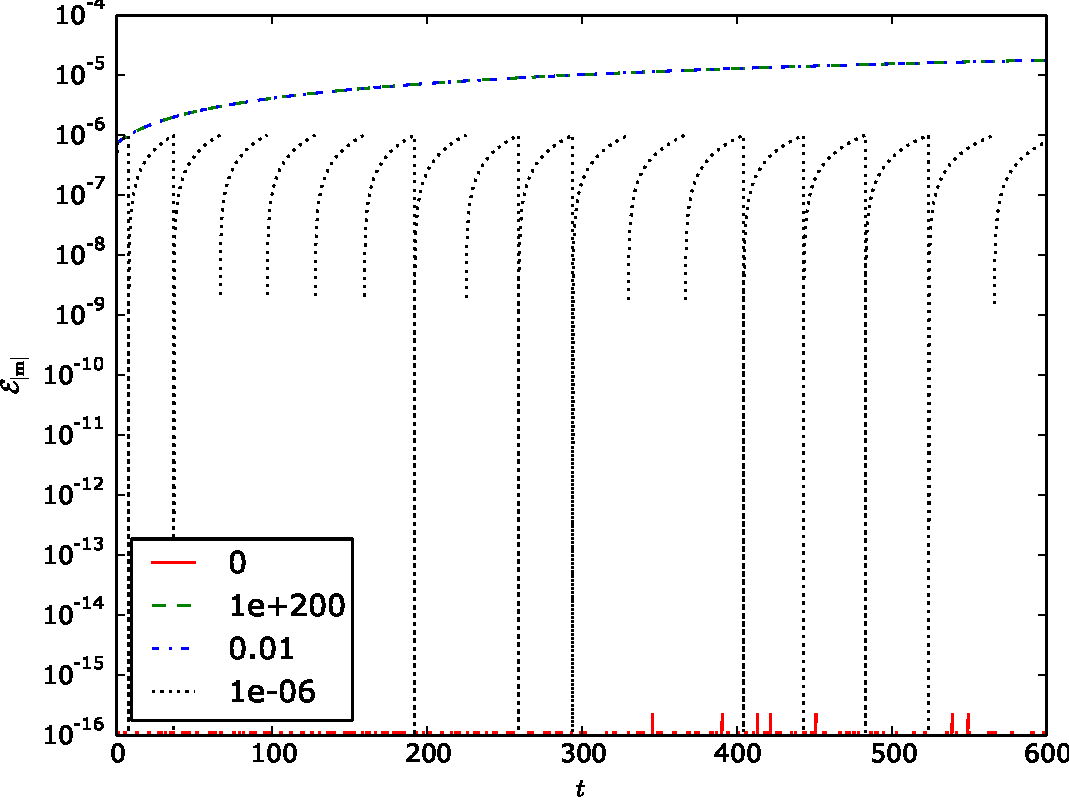
\includegraphics[width=0.8\textwidth]{{{plots//tolrenorm-geom-properties/0-mlengtherrormaxesvstimes}}}
  \caption{
    Error in magnetisation length against time
    for the ODE LLG problem with
    $\dampc = 0$.
    The legend indicates the values of $\mltol$, the tolerance after which the magnetisation is re-normalised.
  }
  \label{fig:renorm-tol-ml-err-undamped}
\end{figure}

In \cref{fig:renorm-tol-ml-err,fig:renorm-tol-ml-err-undamped} we show the error in the magnetisation length over time for various values of $\mltol$ for the damped and undamped problems respectively.
Note that $\mltol = 10^{200}$ results in no renormalisation being carried out ever, while $\mltol = 0$ results in re-normalisation after every time step.
In both the damped and undamped cases, the use of the intermediate tolerance value, $\mltol = 10^{-6}$, results in oscillations of the magnetisation length.
In the undamped case with $\mltol = 10^{-2}$ the error in the magnetisation length never reaches the tolerance, and so the behaviour is identical to no renormalisation.
In the damped case $\mltol = 10^{-2}$ is reached and the behaviour is similar to that of $\mltol = 10^{-6}$, except that the oscillations begin at a later time.

Note that for $\mltol = 10^{-6}$ and times $t \gtrsim 280$ the magnetisation is renormalised after almost every step (hence the small error values).

\begin{figure}
  \centering
  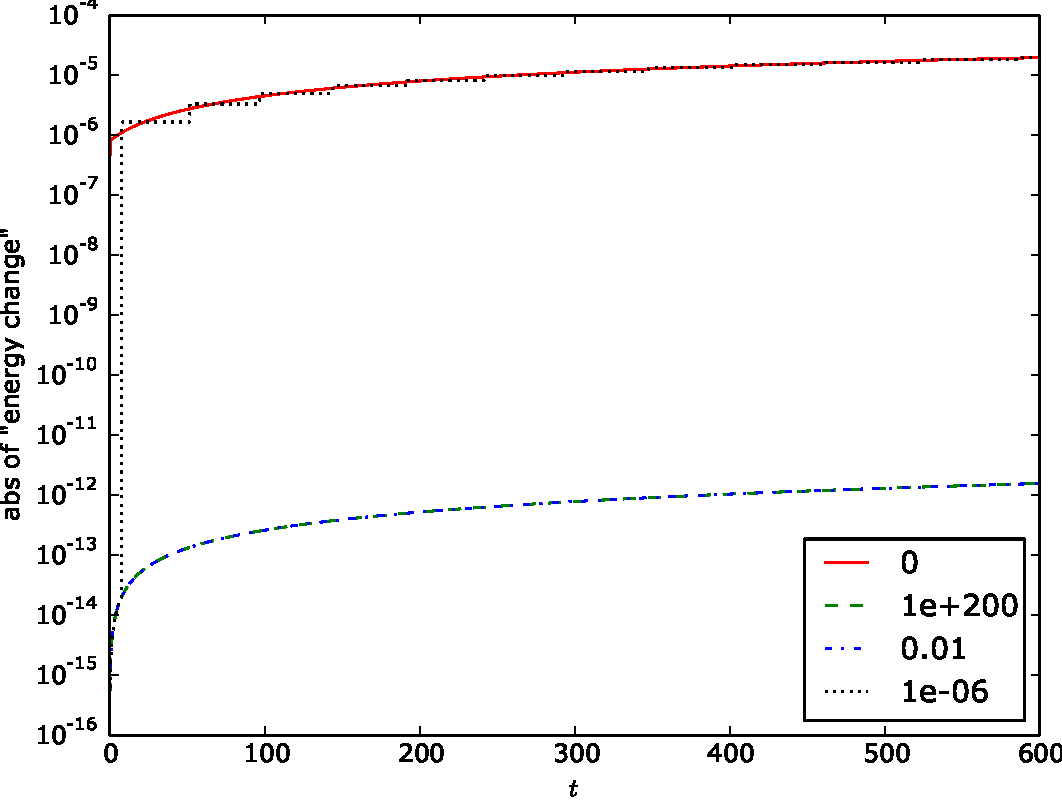
\includegraphics[width=0.8\textwidth]{plots/tolrenorm-geom-properties/0-absofenergychangevstimes.pdf}
  \caption{
    Error in energy against time
    for the ODE LLG problem
    with $\dampc = 0$.
    The legend indicates the values of $\mltol$, the tolerance after which the magnetisation is re-normalised.
  }
  \label{fig:renorm-tol-energy-err}
\end{figure}

In \cref{fig:renorm-tol-energy-err} the errors in the energy for the undamped case are shown.
As noted previously, $\mltol= 10^{-2}$ behaves as the non-renormalised case for this example.
When $\mltol = 10^{-6}$ we see an error similar to that for the always renormalised case, except with additional oscillations in the energy corresponding to times where a renormalisation is carried out.


\begin{figure}
  \centering
  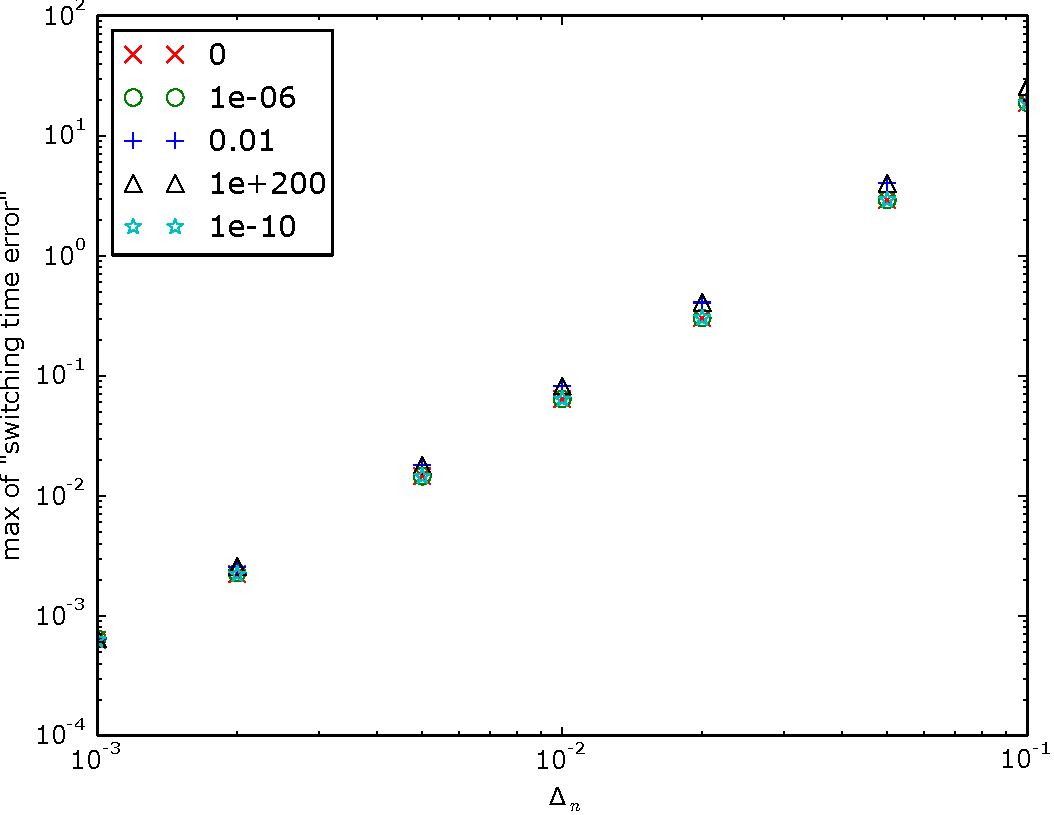
\includegraphics[width=0.8\textwidth]{plots/tolrenorm_llg_ode_convergence/maxofswitchingtimeerrorvsmeanofdts}
  \caption{
    Convergence of the maximum (over all steps) of the error in the switching time
    against step size
    for the ODE LLG problem with
    $\dampc = 0.01$.
    The legend indicates the tolerance after which the magnetisation is re-normalised.
    ??ds not actually a mean...
  }
  \label{fig:tol-renorm-convergence}
\end{figure}

Finally in \cref{fig:tol-renorm-convergence} we show the convergence of the method (in terms of the error in the switching time) for the damped case as the step size is reduced.
It can be seen that the $\mltol=10^{-2}$ or no renormalisation gives slightly worse errors for large step sizes than the tighter magnetisation length tolerances.

??ds add more intermediate tolerances? But we need to output values before renormalising to see anything in this case... I think intermediate tols (less than e-6) are basically the same as always renorm.


\FloatBarrier
\subsection{The self-correcting LLG}
\label{sec:self-correcting-llg-results}

The self correcting parameter $\scc = 0, 0.1, 1, 10, 100, 1000$, larger values were not used because the Newton-Raphson method began to fail to converge within ten steps.


\begin{figure}
  \centering
  \includegraphics[width=0.8\textwidth]{{{plots/sc-geom-properties/0.01-mlengtherrormaxesvstimes}}}
  \caption{
    Error in magnetisation length against time
    for the ODE self-correcting LLG problem
    with $\dampc = 0.01$.
    The legend indicates the values of $\scc$.
  }
  \label{fig:sc-ml-err}
\end{figure}

\begin{figure}
  \centering
  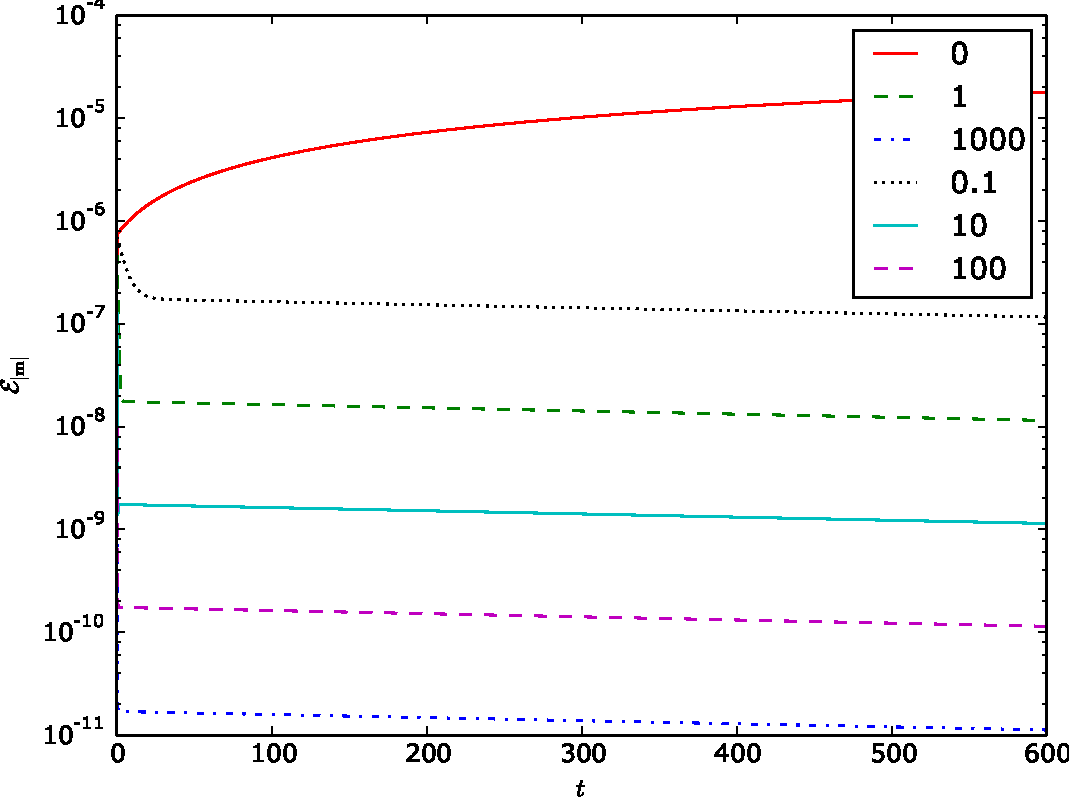
\includegraphics[width=0.8\textwidth]{plots//sc-geom-properties/0-mlengtherrormaxesvstimes.pdf}
  \caption{
    Error in magnetisation length against time
    for the ODE self-correcting LLG problem
    with $\dampc = 0$.
    The legend indicates the values of $\scc$.
  }
  \label{fig:sc-ml-err-undamped}
\end{figure}

In \cref{fig:sc-ml-err,fig:sc-ml-err-undamped} we show the errors in magnetisation length over time for various values of the parameter $\scc$ for the damped and undamped problems respectively.
As would be expected larger values of $\scc$ improve (reduce) the error in both cases.
%??ds what's up with that initial transient...

Note that in the damped case (\cref{fig:sc-ml-err}) with $\scc = 1000$ the curve stops at $t \sim 480$, this is due to the failure of the Newton-Raphson method to converge within the ten steps allowed.
Larger values of $\scc$ resulted in a large number of instances of non-convergence.
Details of the impact of $\scc$ on the Newton-Raphson method will be discussed later.

\begin{figure}
  \centering
  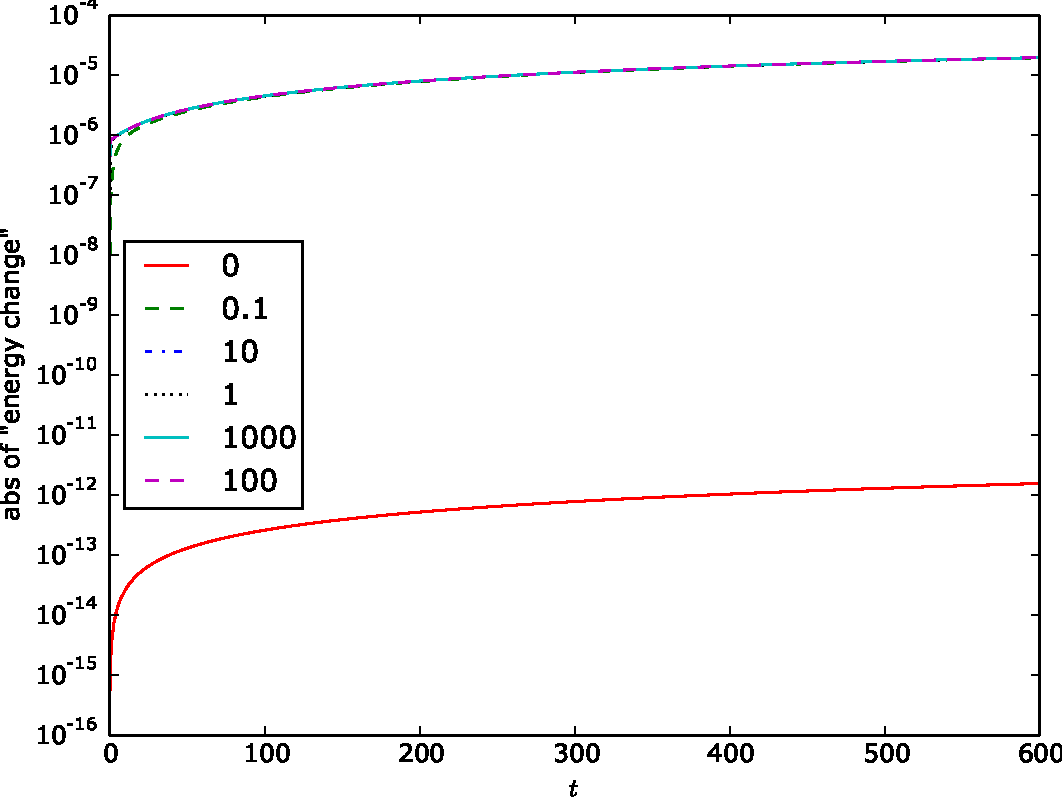
\includegraphics[width=0.8\textwidth]
  {{{plots/sc-geom-properties/0-absofenergychangevstimes}}}
  \caption{
    Error in energy against time
    for the ODE self-correcting LLG problem
    with $\dampc = 0$.
    The legend indicates the values of $\scc$.
  }
  \label{fig:sc-energy-err}
\end{figure}

In \cref{fig:sc-energy-err} we show the error in the energy for the undamped ODE LLG problem with various values of $\scc$.
We see that any $\scc > 0$ causes an error in the energy similarly to the renormalisation approaches shown in \cref{fig:renorm-tol-energy-err}.


\begin{figure}
  \centering
  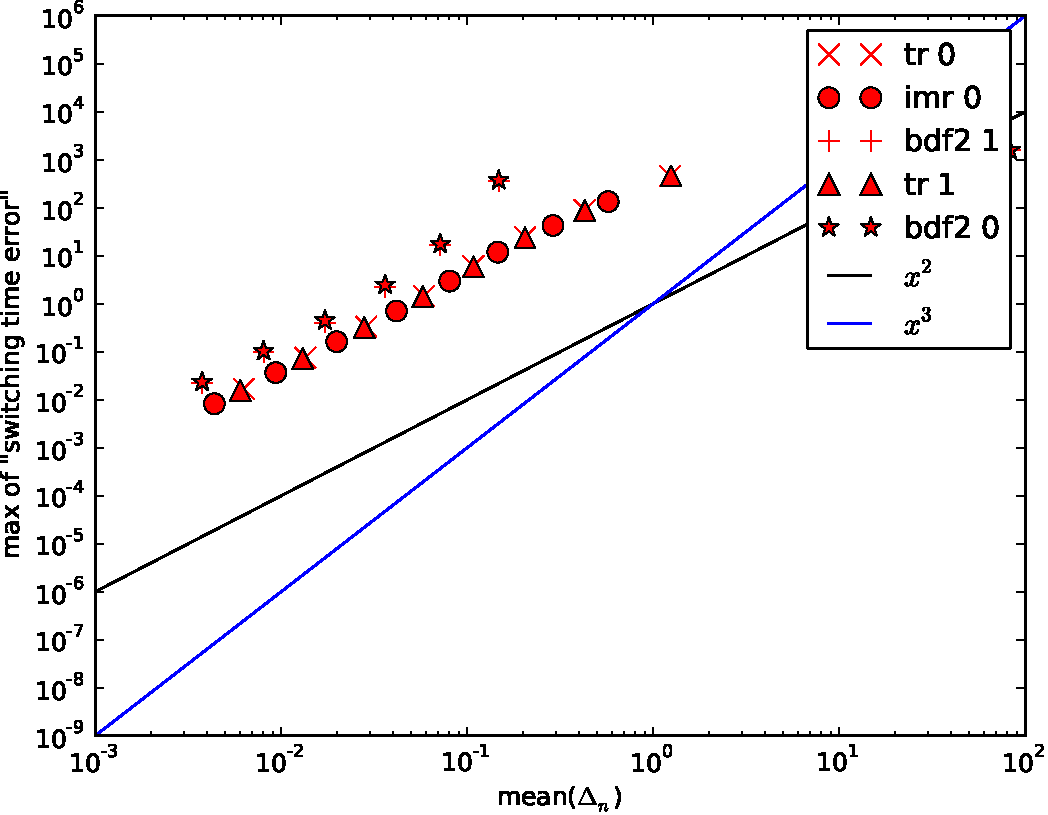
\includegraphics[width=0.8\textwidth]
  {{{plots/self_correcting_llg_ode_convergence/maxofswitchingtimeerrorvsmeanofdts}}}
  \caption{
    Convergence of the maximum (over all steps) of the error in the switching time
    against step size
    for the ODE self-correcting LLG problem with
    $\dampc = 0.01$.
    The legend indicates, respectively, the values of $\scc$ and the tolerance after which the magnetisation is re-normalised.
  }
  \label{fig:sc-convergence}
\end{figure}

In \cref{fig:sc-convergence} we show the convergence of the maximum error in the switching time against the time step size $\dtn$ with two values of $\scc$.
For comparison we also show the results with $\scc = 0$ and re-normalisation after every step (\ie $\mltol = 0$).
We see that the resulting errors are essentially identical for all three cases.

\FloatBarrier % force latex to place all the figures before this table (hacky...)
\begin{table}
  \begin{subtable}{.5\textwidth}
    \centering
    \begin{tabular}{ll}
      $\scc$ & Mean Newton iterations \\
      \hline
      0 & 2.0 \\
      0.1 & 2.0 \\
      1 & 2.46 \\
      10 & 2.68 \\
      100 & 3.13 \\
      1000 & 3.12 \\
    \end{tabular}%
    \caption{Solved with BDF2 and $\ntol = 10^{-8}$}
  \end{subtable}%
  \begin{subtable}{.5\textwidth}
    \centering
    \begin{tabular}{ll}
      $\scc$ & Mean Newton iterations \\
      \hline
      0 & 2.0 \\
      0.1 & - \\
      1 & - \\
      10 & - \\
      100 & - \\
      1000 & - \\
    \end{tabular}%
    \vfill
    \caption{Solved with IMR and $\ntol = 10^{-12}$}
  \end{subtable}%
  \caption{
    Mean (over all time steps) number of Newton iterations for convergences
    for the ODE self-correcting LLG problem with
    $\dampc = 0.01$.
    The numerical methods used are indicated in the sub-captions.
    Values of $\scc \neq 0$ are not considered when using IMR because no self-correcting term is needed to conserve $\abs{\mv}$.
  }
  \label{tab:sc-newton-iters}
\end{table}


In \cref{tab:sc-newton-iters} we show the number of Newton-Raphson iterations required for convergence.
For comparison we also show plots using IMR, with Newton tolerance $\ntol=10^{-12}$ (recall that a sharp linearisation tolerance is required for IMR to attain good geometric integration properties).
We see that for larger values of $\scc$ additional iterations are required.
In addition we see that the tighter tolerance required for geometric integration with IMR has no effect on the number of iterations.

Since $\scc \geq 100$ is required to control $\errml$ to even the fairly loose level of $10^{-6}$ in the (very simple) example of the damped ODE problem, we can conclude that use of the self correcting term will require at least one additional Newton-Raphson iteration.

As the majority of the computation time for a time step is spent within the Newton-Raphson method, this increased the cost of each step by a factor of approximately $3/2$.
Since the use of the self-correcting method does not provide any improvement in the overall accuracy over always re-normalising (so the same $\dtn$ is required to obtain the same accuracy), this increases the overall cost of the method by the same factor.



\subsection{Conclusions}

Renormalisation after a tolerance allows larger errors in $\abs{\mv}$ than renorm after each step (by definition).
It also introduces spurious oscillations in $\abs{\mv}$.
It has a slight negative effect on convergence when compared to re-normalisation after every step.
In terms of computational cost: checking whether renormalisation is needed has roughly the same cost as actually re-normalising.
Hence there is no reason to prefer renormalisation after a tolerance.

Self correcting LLG is always worse in controlling GI errors than renorm after each step: energy errors the same, m errors much larger.
It also takes additional newton step(s) (typically one more step is needed, increasing the computational time for the simulation by a factor of $\sim 3/2$).
It gives essentially identical convergence properties as re-normalisation after every step.
As such there is no reason to use the self-correcting LLG over renormalisation after each step.

%%% Local Variables:
%%% mode: latex
%%% TeX-master: "main"
%%% End:
